%% LyX 1.3 created this file.  For more info, see http://www.lyx.org/.
%% Do not edit unless you really know what you are doing.
\documentclass[english, 12pt]{article}
\usepackage{times}
%\usepackage{algorithm2e}
\usepackage{url}
\usepackage{bbm}
\usepackage[T1]{fontenc}
\usepackage[latin1]{inputenc}
\usepackage{geometry}
\geometry{verbose,letterpaper,tmargin=2cm,bmargin=2cm,lmargin=1.5cm,rmargin=1.5cm}
\usepackage{rotating}
\usepackage{color}
\usepackage{graphicx}
\usepackage{subcaption}
\usepackage{amsmath, amsthm, amssymb}
\usepackage{setspace}
\usepackage{lineno}
\usepackage{hyperref}
\usepackage{bbm}
\usepackage{makecell}

%\renewcommand{\arraystretch}{1.8}

%\usepackage{xr}
%\externaldocument{SCT-supp}

%\linenumbers
%\doublespacing
\onehalfspacing
%\usepackage[authoryear]{natbib}
\usepackage{natbib} \bibpunct{(}{)}{;}{author-year}{}{,}

%Pour les rajouts
\usepackage{color}
\definecolor{trustcolor}{rgb}{0,0,1}

\usepackage{dsfont}
\usepackage[warn]{textcomp}
\usepackage{adjustbox}
\usepackage{multirow}
\usepackage{graphicx}
\graphicspath{{figures/}}
\DeclareMathOperator*{\argmin}{\arg\!\min}

\let\tabbeg\tabular
\let\tabend\endtabular
\renewenvironment{tabular}{\begin{adjustbox}{max width=0.9\textwidth}\tabbeg}{\tabend\end{adjustbox}}

\makeatletter

%%%%%%%%%%%%%%%%%%%%%%%%%%%%%% LyX specific LaTeX commands.
%% Bold symbol macro for standard LaTeX users
%\newcommand{\boldsymbol}[1]{\mbox{\boldmath $#1$}}

%% Because html converters don't know tabularnewline
\providecommand{\tabularnewline}{\\}

\usepackage{babel}
\makeatother


\begin{document}


\title{Supplementary Note}

\date{~ }
\maketitle


%%%%%%%%%%%%%%%%%%%%%%%%%%%%%%%%%%%%%%%%%%%%%%%%%%%%%%%%%%%%%%%%%%%%%%%%%%%%%%%%

\section*{Version 4 of pcadapt provides similar results as previous versions}

\renewcommand{\thefigure}{S\arabic{figure}}
\setcounter{figure}{0}
\renewcommand{\thetable}{S\arabic{table}}
\setcounter{table}{0}

There are two main differences between version 4 of pcadapt and its previous versions.
First, R package pcadapt now uses PLINK format `bed' instead of format `pcadapt'. Both formats store the same data, i.e.\ genotype calls 0, 1, or 2, and missing values. Thus, changing the preferred format in pcadapt has no impact on results.

Second, pcadapt now uses a different way to compute top Principal Components (PCs) of the genotype matrix.
While computed PCs should be similar when there is no missing value, we changed how we handle missing values in version 4 of pcadapt.
Computing PCs in previous versions relied on computing the Genetic Relationship Matrix (GRM). When there were missing values, only pairwise complete observations were used to compute the GRM, i.e.\
\begin{equation}
\text{GRM}_{ij} = \frac{1}{\sum_{k=1}^p \delta_{ik}\delta_{jk}} \sum_{k = 1}^p \widetilde{G}_{ik} ~ \widetilde{G}_{jk} ~ \delta_{ik} ~ \delta_{jk}~,
\end{equation}
where $\widetilde{G}$ is the scaled genotype matrix and $\delta_{ik}$ is an indicator if the genotype for individual $i$ and variant $k$ is available ($\delta_{ik} = 1$) or missing ($\delta_{ik} = 0$).
To compute PCs in pcadapt v4, we now rely on a faster truncated Singular Value Decomposition algorithm that does not require computing the GRM. 
This algorithm only needs a function that computes the product and cross-product of the (scaled) genotype matrix with a given vector.
To allow for missing values, we compute
\begin{equation}
\begin{split}
\forall j \in [|1,p|], \; \left(\widetilde{G}^T x\right)_j &= \frac{n}{\sum_{i=1}^n \delta_{ij}} \sum_{i = 1}^n \widetilde{G}_{ij} ~ \delta_{ij} ~ x_i,  \\
\forall i \in [|1,n|], \; \left(\widetilde{G} y\right)_i &= \frac{p}{\sum_{j=1}^p \delta_{ij}} \sum_{j = 1}^p \widetilde{G}_{ij} ~ \delta_{ij} ~ y_j.
\end{split}
\end{equation}

To compare resulting chi-square statistics between versions of pcadapt, we use the same data of domestic dogs that we used for timing comparisons.
This dataset contains a small number of missing values only. We artificially create 5 new genotype matrices where we add missing values.
We simulate the number of missing values per variant using a beta-binomial distribution.
Then, for each variant, we randomly assign as missing the given number of genotypes.
This results in datasets with approximately 21\% missing values on average with a wide range of number of missing values per variant, i.e.\  possibly ranging from none to all missing.
When running old (v3.0.4) and new (v4.1.0) versions of pcadapt on these datasets with a large number of missing values, we find that both versions provide very similar results, with correlations between chi-square statistics always larger than 0.997 (Figure \ref{fig:corstats}).

To conclude, version 4 of pcadapt provides almost unchanged results compared to previous versions, even where there is 21\% of missing values in the data. 

%%%%%%%%%%%%%%%%%%%%%%%%%%%%%%%%%%%%%%%%%%%%%%%%%%%%%%%%%%%%%%%%%%%%%%%%%%%%%%%%

\begin{figure}[!htpb]
	\centerline{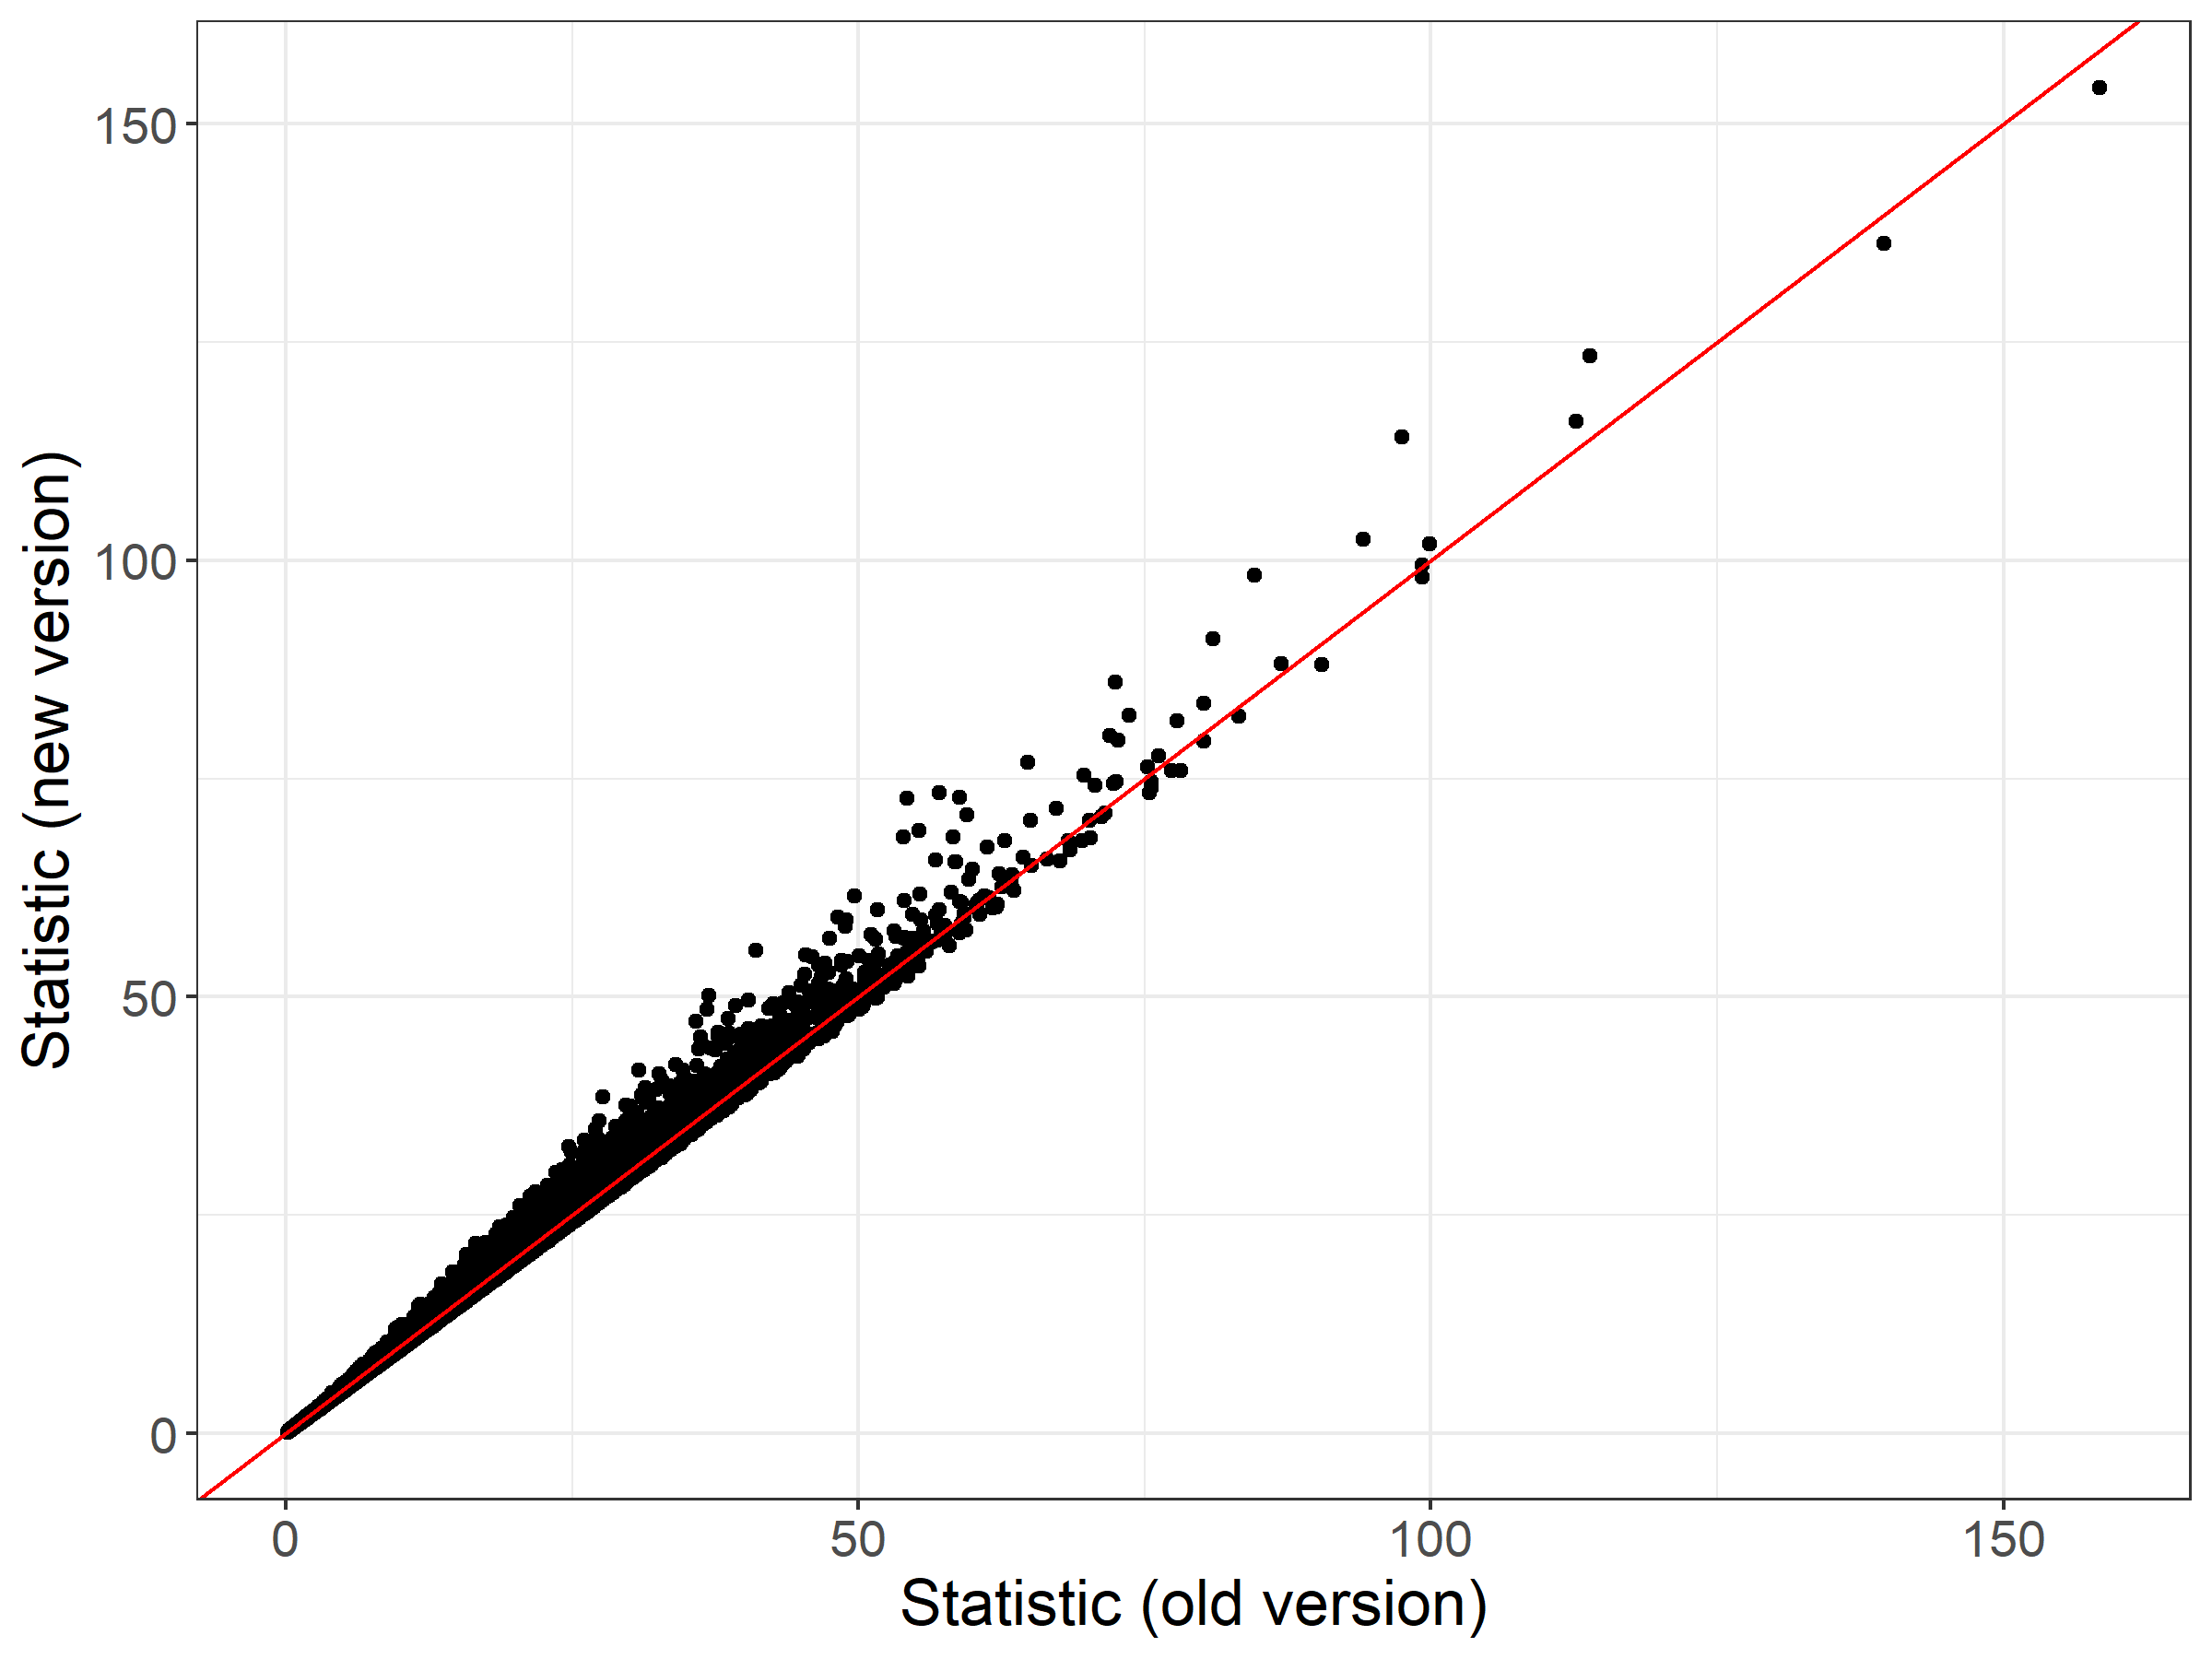
\includegraphics[width=0.75\textwidth]{compare-with-old.png}}
	\caption{For one dataset with a large number of missing values, chi-square statistics from pcadapt v4.1.0 (y-axis) versus statistics from v3.0.4 (x-axis). Correlation between these statistics is of 99.76\%. \label{fig:corstats}}
\end{figure}

%%%%%%%%%%%%%%%%%%%%%%%%%%%%%%%%%%%%%%%%%%%%%%%%%%%%%%%%%%%%%%%%%%%%%%%%%%%%%%%%

\end{document}
